% Diagrama E — similaridade progressiva de N*: prefixos crescentes da grade,
% matrizes dirigidas recomputadas e comparação em duas componentes.
\documentclass[tikz,border=6pt]{standalone}
% Preâmbulo compartilhado dos diagramas conceituais do relatório CoInfoSim.
% Compilação: xelatex (determinística; nenhum dado experimental é usado).
\usepackage{fontspec}
\setmainfont{Liberation Sans}
\setsansfont{Liberation Sans}
\usepackage{amsmath}
\usepackage{bm}
\usepackage{tikz}
\usetikzlibrary{arrows.meta,positioning,calc,fit,backgrounds,decorations.pathreplacing,matrix,patterns}
\definecolor{CoinAccent}{RGB}{25,80,140}
\definecolor{CoinAccentDark}{RGB}{18,55,95}
\definecolor{CoinAccentPale}{RGB}{237,242,248}
\definecolor{CoinGray}{RGB}{95,95,95}
\definecolor{CoinGrayPale}{RGB}{246,246,246}
\definecolor{CoinWin}{RGB}{76,140,90}    % verde discreto (vitória)
\definecolor{CoinLose}{RGB}{182,88,79}   % vermelho discreto (derrota)
\tikzset{
  bloco/.style={draw=CoinAccentDark, fill=CoinAccentPale, rounded corners=1.2pt,
                align=center, font=\small, inner sep=4pt, minimum height=7mm},
  bloconeutro/.style={draw=CoinGray, fill=CoinGrayPale, rounded corners=1.2pt,
                align=center, font=\small, inner sep=4pt, minimum height=7mm},
  blocoreal/.style={draw=CoinAccentDark, fill=white, rounded corners=1.2pt,
                align=center, font=\small, inner sep=4pt, minimum height=7mm},
  seta/.style={-{Stealth[length=2.4mm]}, thick, CoinAccentDark},
  setacinza/.style={-{Stealth[length=2.4mm]}, thick, CoinGray},
  rotulo/.style={font=\footnotesize\itshape, text=CoinGray, align=center},
}

\begin{document}
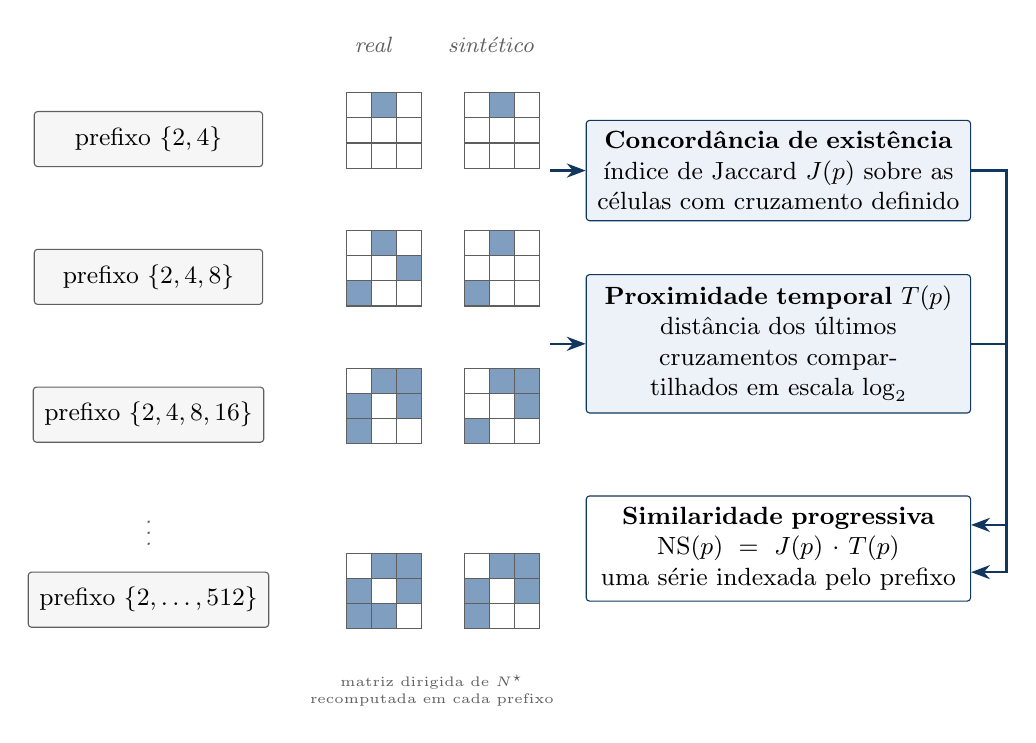
\begin{tikzpicture}[node distance=4mm]
  \tikzset{mini/.style={draw=CoinGray, minimum size=3.2mm, inner sep=0pt, font=\tiny}}

  % Função auxiliar visual: mini-matriz 3x3 dirigida (células preenchidas = N* definido)
  \newcommand{\minimatriz}[3]{% x, y, lista de células preenchidas r/c
    \begin{scope}[shift={(#1,#2)}]
      \foreach \r in {1,2,3}\foreach \c in {1,2,3}{
        \node[mini] at (\c*0.32,-\r*0.32) {};
      }
      \foreach \r/\c in {#3}{
        \node[mini, fill=CoinAccent!55] at (\c*0.32,-\r*0.32) {};
      }
    \end{scope}}

  % Linhas de prefixo
  \foreach \i/\pref in {0/{$\{2,4\}$}, 1/{$\{2,4,8\}$}, 2/{$\{2,4,8,16\}$}}{
    \node[bloconeutro, minimum width=2.9cm, font=\small] (p\i) at (0,-\i*1.75) {prefixo \pref};
  }
  \node[rotulo] (dots) at (0,-3*1.75+0.35) {$\vdots$};
  \node[bloconeutro, minimum width=2.9cm, font=\small] (pfim) at (0,-3*1.75-0.6) {prefixo $\{2,\ldots,512\}$};

  % Matrizes real/sintética por prefixo (densidade cresce com o prefixo)
  \minimatriz{2.35}{0.75}{1/2}
  \minimatriz{3.85}{0.75}{1/2}
  \minimatriz{2.35}{-1.0}{1/2,2/3,3/1}
  \minimatriz{3.85}{-1.0}{1/2,3/1}
  \minimatriz{2.35}{-2.75}{1/2,2/3,3/1,1/3,2/1}
  \minimatriz{3.85}{-2.75}{1/2,2/3,3/1,1/3}
  \minimatriz{2.35}{-5.1}{1/2,2/3,3/1,1/3,2/1,3/2}
  \minimatriz{3.85}{-5.1}{1/2,2/3,3/1,1/3,2/1}

  \node[rotulo] at (2.85,1.2) {real};
  \node[rotulo] at (4.35,1.2) {sintético};
  \node[rotulo, text width=3.2cm, font=\tiny] at (3.6,-7.0)
    {matriz dirigida de $N^{\star}$\\recomputada em cada prefixo};

  % Comparação (duas componentes) e produto
  \node[bloco, text width=4.6cm, font=\small] (jac) at (8.0,-0.4)
    {\textbf{Concordância de existência}\\índice de Jaccard $J(p)$ sobre as células com cruzamento definido};
  \node[bloco, text width=4.6cm, font=\small] (tim) at (8.0,-2.6)
    {\textbf{Proximidade temporal} $T(p)$\\distância dos últimos cruzamentos compartilhados em escala $\log_2$};
  \node[bloco, text width=4.6cm, font=\small, fill=white] (ns) at (8.0,-5.2)
    {\textbf{Similaridade progressiva}\\$\mathrm{NS}(p)=J(p)\cdot T(p)$\\uma série indexada pelo prefixo};

  \draw[seta] (5.1,-0.4) -- (jac.west);
  \draw[seta] (5.1,-2.6) -- (tim.west);
  \draw[seta] (jac.east) -- ++(0.45,0) |- ($(ns.east)+(0.0,0.30)$);
  \draw[seta] (tim.east) -- ++(0.45,0) |- ($(ns.east)+(0.0,-0.30)$);
\end{tikzpicture}
\end{document}
